\documentclass[main.tex]{subfiles}

%TODO remove
%%tikz
\usepackage{tikz}
\usetikzlibrary{knots, cd, calc}



\newcommand{\coxtwothreethree}{%
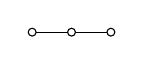
\begin{tikzpicture}[scale=0.5]
\draw (0, 0) circle (0.1);
\draw (1, 0) circle (0.1);
\draw (2, 0) circle (0.1);
\draw (0.1, 0) -- (0.9, 0);
\draw (1.1, 0) -- (1.9, 0);
\end{tikzpicture}}

\newcommand{\coxthreethreethree}{%
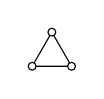
\begin{tikzpicture}[scale = 0.5]
\draw (0, 0) -- (60:1) -- (1, 0) -- (0, 0);
\draw[fill = white] (0, 0) circle (0.1);
\draw[fill = white] (60:1) circle (0.1);
\draw[fill = white] (1, 0) circle (0.1);
\end{tikzpicture}}

\newcommand{\coxthreethreethreetype}[1]{%
\begin{tikzpicture}[scale = 0.5]
\draw (0, 0) -- (60:1) -- (1, 0) -- (0, 0);
\draw[fill = white] (0, 0) circle (0.1);
\draw[fill = white] (60:1) circle (0.1);
\draw[fill = white] (1, 0) circle (0.1);
\node at (0.5, 0.2) {\tiny{#1}};
\end{tikzpicture}}

\newcommand{\coxathreetype}[1]{%
\begin{tikzpicture}[scale=0.5]
\draw (0, 0) circle (0.1);
\draw (1, 0) circle (0.1);
\draw (2, 0) circle (0.1);
\draw (0.1, 0) -- (0.9, 0);
\draw (1.1, 0) -- (1.9, 0);

\node at (0.5, 0.2) {\tiny{#1}};
\end{tikzpicture}}

\newcommand{\coxathreetypedouble}[2]{%
\begin{tikzpicture}[scale=0.5]
\draw (0, 0) circle (0.1);
\draw (1, 0) circle (0.1);
\draw (2, 0) circle (0.1);
\draw (0.1, 0) -- (0.9, 0);
\draw (1.1, 0) -- (1.9, 0);

\node at (0.5, 0.2) {\tiny{#1}};
\node at (1.5, 0.2) {\tiny{#2}};
\end{tikzpicture}}

\newcommand{\coxfourthreethree}{%
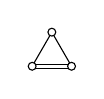
\begin{tikzpicture}[scale = 0.5]
\draw (0, 0) -- (60:1) -- (1, 0);
\draw (0, 0.05) -- (1, 0.05);
\draw (0, -0.05) -- (1, -0.05);
\draw[fill = white] (0, 0) circle (0.1);
\draw[fill = white] (60:1) circle (0.1);
\draw[fill = white] (1, 0) circle (0.1);
\end{tikzpicture}
}


\begin{document}
\section{Appendix}\label{sec:data}
Table \ref{tab:cox-quotients-10-crossings} consists of the Coxeter quotients we found for three-bridge knots of crossing number $10$. It was computed using the same algorithm as in Section \ref{subsec:list-of-quotients}. No quotients were found for $10_{79}, 10_{80}, 10_{81}, 
10_{83}$, $10_{86}$, $10_{88}$, $10_{89}$, $10_{91}$, $10_{92}$, $10_{94}$, $10_{95}$, $10_{96}$, $10_{97}$,
$10_{100}$, $10_{101}$, $10_{103}$, $10_{104}$, $10_{105}$, $10_{106}$, $10_{107}$, $10_{109}$, $10_{110}$, $10_{111}$, $10_{114}$, $10_{115}$, $10_{116}$, $10_{117}$, $10_{118}$, $10_{119}$, $10_{121}$, $10_{122}$, $10_{123}$,
$10_{148}$, $10_{149}$, $10_{150}$, $10_{151}$, $10_{152}$, $10_{153}$, $10_{154}$, $10_{155}$, $10_{156}$, $10_{158}$,
$10_{160}$, $10_{161}$, $10_{162}$ and $10_{163}$. The knots that are not mentioned are two-bridge knots.

\begin{table}[htb]
\newcommand{\correctspace}{$\;\;\,$}
\centering
\begin{minipage}[t]{0.5\textwidth}
\centering
\begin{tabular}[t]{c|c}
Knot & Coxeter Quotients \\
\hline
\verticalcenter{$10_{46}$} & \verticalcenter{\includegraphics{dynkin-diagrams/h_3}} \\
\verticalcenter{$10_{47}$} & \verticalcenter{\includegraphics{dynkin-diagrams/h_3}} \\
\verticalcenter{$10_{48}$} & \verticalcenter{\includegraphics{dynkin-diagrams/h_3}} \\
\verticalcenter{$10_{49}$} & \verticalcenter{\includegraphics{dynkin-diagrams/h_3}} \\
\verticalcenter{$10_{50}$} & \verticalcenter{\includegraphics{dynkin-diagrams/(2,3,7)}} \\
\verticalcenter{$10_{51}$} & \verticalcenter{\includegraphics{dynkin-diagrams/(2,3,7)}} \\
\verticalcenter{$10_{52}$} & \verticalcenter{\includegraphics{dynkin-diagrams/(2,3,7)}} \\
\verticalcenter{$10_{53}$} & \verticalcenter{\includegraphics{dynkin-diagrams/(2,3,7)}} \\
\verticalcenter{$10_{54}$} & \verticalcenter{\includegraphics{dynkin-diagrams/(2,3,7)}} \\
\verticalcenter{$10_{55}$} & \verticalcenter{\includegraphics{dynkin-diagrams/(2,3,7)}} \\
\verticalcenter{$10_{56}$} & \verticalcenter{\includegraphics{dynkin-diagrams/(2,3,7)}} \\
\verticalcenter{$10_{57}$} & \verticalcenter{\includegraphics{dynkin-diagrams/(2,3,7)}} \\
\verticalcenter{$10_{58}$} & \correctspace\verticalcenter{\verticalcenter{\includegraphics{dynkin-diagrams/h_3}} and \verticalcenter{\includegraphics{dynkin-diagrams/(2,5,5)}}} \\ 
\verticalcenter{$10_{59}$} & \correctspace\verticalcenter{\verticalcenter{\includegraphics{dynkin-diagrams/h_3}} and \verticalcenter{\includegraphics{dynkin-diagrams/(2,5,5)}}} \\ 
\verticalcenter{$10_{60}$} & \correctspace\verticalcenter{\verticalcenter{\includegraphics{dynkin-diagrams/h_3}} and \verticalcenter{\includegraphics{dynkin-diagrams/(2,5,5)}}} \\ 
\verticalcenter{$10_{61}$} & \verticalcenter{\includegraphics{dynkin-diagrams/(3,3,4)}} \\
\verticalcenter{$10_{62}$} & \verticalcenter{\includegraphics{dynkin-diagrams/(3,3,4)}} \\
\verticalcenter{$10_{63}$} & \verticalcenter{\includegraphics{dynkin-diagrams/(3,3,4)}} \\
\verticalcenter{$10_{64}$} & \verticalcenter{\includegraphics{dynkin-diagrams/(3,3,4)}} \\
\verticalcenter{$10_{65}$} & \verticalcenter{\includegraphics{dynkin-diagrams/(3,3,4)}} \\
\verticalcenter{$10_{66}$} & \verticalcenter{\includegraphics{dynkin-diagrams/(3,3,4)}} \\
\verticalcenter{$10_{67}$} & \verticalcenter{\verticalcenter{\includegraphics{dynkin-diagrams/h_3}} and \verticalcenter{\includegraphics{dynkin-diagrams/(3,3,5)}}} \\
\verticalcenter{$10_{68}$} & \verticalcenter{\verticalcenter{\includegraphics{dynkin-diagrams/h_3}} and \verticalcenter{\includegraphics{dynkin-diagrams/(3,3,5)}}} \\
\verticalcenter{$10_{69}$} & \verticalcenter{\verticalcenter{\includegraphics{dynkin-diagrams/h_3}} and \verticalcenter{\includegraphics{dynkin-diagrams/(3,3,5)}}} \\
\verticalcenter{$10_{70}$} & \verticalcenter{\includegraphics{dynkin-diagrams/h_3}} \\
\verticalcenter{$10_{71}$} & \verticalcenter{\includegraphics{dynkin-diagrams/h_3}} \\
\verticalcenter{$10_{72}$} & \verticalcenter{\includegraphics{dynkin-diagrams/h_3}} \\
\verticalcenter{$10_{73}$} & \verticalcenter{\includegraphics{dynkin-diagrams/h_3}} \\
\verticalcenter{$10_{76}$} & \verticalcenter{\includegraphics{dynkin-diagrams/a_3}} \\
\verticalcenter{$10_{77}$} & \verticalcenter{\includegraphics{dynkin-diagrams/a_3}} \\
\verticalcenter{$10_{78}$} & \verticalcenter{\includegraphics{dynkin-diagrams/a_3}} \\
\verticalcenter{$10_{82}$} & \verticalcenter{\includegraphics{dynkin-diagrams/a_3}} \\
\verticalcenter{$10_{84}$} & \verticalcenter{\includegraphics{dynkin-diagrams/a_3}} \\
\verticalcenter{$10_{85}$} & \verticalcenter{\includegraphics{dynkin-diagrams/a_3}} \\
\verticalcenter{$10_{87}$} & \verticalcenter{\includegraphics{dynkin-diagrams/a_3}} \\
\verticalcenter{$10_{90}$} & \verticalcenter{\includegraphics{dynkin-diagrams/h_3}} \\
\verticalcenter{$10_{93}$} & \verticalcenter{\includegraphics{dynkin-diagrams/h_3}} \\
\end{tabular}
\end{minipage}%
\begin{minipage}[t]{0.5\textwidth}
\centering
\begin{tabular}[t]{c|c}
Knot & Coxeter Quotients \\
\hline
\verticalcenter{$10_{98}$}\rule{0pt}{4ex} & \verticalcenter{\verticalcenter{\includegraphics{dynkin-diagrams/h_3}} and \verticalcenter{\includegraphics{dynkin-diagrams/(3,3,inf)}}} \\
\verticalcenter{$10_{99}$} & \verticalcenter{\verticalcenter{\includegraphics{dynkin-diagrams/h_3}} and \verticalcenter{\includegraphics{dynkin-diagrams/(3,3,inf)}}} \\
\verticalcenter{$10_{102}$} & \verticalcenter{\includegraphics{dynkin-diagrams/h_3}} \\
\verticalcenter{$10_{108}$} & \verticalcenter{\includegraphics{dynkin-diagrams/h_3}} \\
\verticalcenter{$10_{112}$} & \verticalcenter{\includegraphics{dynkin-diagrams/h_3}} \\\verticalcenter{$10_{113}$} & \verticalcenter{\includegraphics{dynkin-diagrams/h_3}} \\
\verticalcenter{$10_{120}$} & \verticalcenter{\includegraphics{dynkin-diagrams/a_3}} \\
\verticalcenter{$10_{124}$} & \verticalcenter{\includegraphics{dynkin-diagrams/h_3}} \\
\verticalcenter{$10_{125}$} & \verticalcenter{\includegraphics{dynkin-diagrams/h_3}} \\
\verticalcenter{$10_{126}$} & \verticalcenter{\includegraphics{dynkin-diagrams/h_3}} \\
\verticalcenter{$10_{127}$} & \verticalcenter{\includegraphics{dynkin-diagrams/h_3}} \\
\verticalcenter{$10_{128}$} & \verticalcenter{\includegraphics{dynkin-diagrams/(2,3,7)}} \\
\verticalcenter{$10_{129}$} & \verticalcenter{\includegraphics{dynkin-diagrams/(2,3,7)}} \\
\verticalcenter{$10_{130}$} & \verticalcenter{\includegraphics{dynkin-diagrams/(2,3,7)}} \\
\verticalcenter{$10_{131}$} & \verticalcenter{\includegraphics{dynkin-diagrams/(2,3,7)}} \\
\verticalcenter{$10_{132}$} & \verticalcenter{\includegraphics{dynkin-diagrams/(2,3,7)}} \\
\verticalcenter{$10_{133}$} & \verticalcenter{\includegraphics{dynkin-diagrams/(2,3,7)}} \\
\verticalcenter{$10_{134}$} & \verticalcenter{\includegraphics{dynkin-diagrams/(2,3,7)}} \\
\verticalcenter{$10_{135}$} & \verticalcenter{\includegraphics{dynkin-diagrams/(2,3,7)}} \\
\verticalcenter{$10_{136}$} & \correctspace\verticalcenter{\verticalcenter{\includegraphics{dynkin-diagrams/h_3}} and \verticalcenter{\includegraphics{dynkin-diagrams/(2,5,5)}}} \\
\verticalcenter{$10_{137}$} & \correctspace\verticalcenter{\verticalcenter{\includegraphics{dynkin-diagrams/h_3}} and \verticalcenter{\includegraphics{dynkin-diagrams/(2,5,5)}}} \\
\verticalcenter{$10_{138}$} & \correctspace\verticalcenter{\verticalcenter{\includegraphics{dynkin-diagrams/h_3}} and \verticalcenter{\includegraphics{dynkin-diagrams/(2,5,5)}}} \\
\verticalcenter{$10_{139}$} & \verticalcenter{\includegraphics{dynkin-diagrams/(3,3,4)}} \\
\verticalcenter{$10_{140}$} & \verticalcenter{\includegraphics{dynkin-diagrams/(3,3,4)}} \\
\verticalcenter{$10_{141}$} & \verticalcenter{\includegraphics{dynkin-diagrams/(3,3,4)}} \\
\verticalcenter{$10_{142}$} & \verticalcenter{\includegraphics{dynkin-diagrams/(3,3,4)}} \\
\verticalcenter{$10_{143}$} & \verticalcenter{\includegraphics{dynkin-diagrams/(3,3,4)}} \\
\verticalcenter{$10_{144}$} & \verticalcenter{\includegraphics{dynkin-diagrams/(3,3,4)}} \\
\verticalcenter{$10_{145}$} & \verticalcenter{\includegraphics{dynkin-diagrams/h_3}} \\
\verticalcenter{$10_{146}$} & \verticalcenter{\verticalcenter{\includegraphics{dynkin-diagrams/h_3}} and \verticalcenter{\includegraphics{dynkin-diagrams/(3,3,5)}}} \\\verticalcenter{$10_{147}$} & \verticalcenter{\verticalcenter{\includegraphics{dynkin-diagrams/h_3}} and \verticalcenter{\includegraphics{dynkin-diagrams/(3,3,5)}}} \\
\verticalcenter{$10_{157}$} & \verticalcenter{\includegraphics{dynkin-diagrams/h_3}} \\
\verticalcenter{$10_{159}$} & \verticalcenter{\includegraphics{dynkin-diagrams/h_3}} \\
\verticalcenter{$10_{164}$} & \verticalcenter{\includegraphics{dynkin-diagrams/a_3}} \\ \verticalcenter{$10_{165}$} & \verticalcenter{\includegraphics{dynkin-diagrams/a_3}}
\end{tabular}
\end{minipage}
\caption{List of Coxeter knots with bridge index $3$ and crossing number $10$}
\label{tab:cox-quotients-10-crossings}
\end{table}

\newpage

\end{document}